\section{Evaluation} \label{Evaluation}

Having developed a fully functional ByzCoin Blockchain which keeps immutable data about vehicles, leads us to testing our solution in a larger network with different number of conodes and also distinct number of concurrent transactions.\\
\newline
As hardware for our simulations we used the IC Cluster (\url{https://iccluster.epfl.ch}) at EPFL. Depending on the configuration, some nodes might need to be run on a same physical server. Controlling the bandwidth and delay of the network, not only between the servers, but also between every virtual node, is done thanks to the Mininet \cite{Mininet} platform. Each server has 24 cores, 2.5 GHz processor and 256GB of RAM and can run around 300 cothority nodes simultaneously \cite{Mininet}.\\
\newline
When running a simulation, a configuration file is needed. It should contain specific parameters like the name of the simulation, the number of: servers, hosts, transactions etc, as well as the before mentioned delay and bandwidth between nodes.\\
\newline
For our experiments, we needed to implement the \textbf{onet.Simulation} \cite{Onet Simulation} interface, and specify in the \textbf{Run()} method what scenario should happen. In the beginning, it is mandatory to create the genesis block, and set the blockchain up by specifying the time interval for creating blocks and generating the collective distributed key for Calypso \cite{Calypso}. Part of the preparation is also enrolling the administrator and a user that will take the roles of owner, potential buyer and garage mechanic for simplicity.\\
\newline
Next step is deciding which measurements we are interested in. For each one of these measurements, we store in a .csv file the wall time (number of seconds it takes in real life, with the network communication included) and also the system cost calculated in seconds (time during which the system nodes utilize their CPUs).\\
\newline
First, we want to determine the time it takes to concurrently enroll a certain number of cars (defined in the configuration file). Registering vehicles consists of two different transactions: one for creating car DARCs that manage the access policies and another for creating car Instances in the global state.\\
\newline
Furthermore, we measure the time needed to add reports in parallel for each one of the registered cars. This is also done with two transactions by producing first Calypso Write Instances and then updating the car instances to contain the report with the secret data.\\
\newline
Finally, we record how long it takes to read the maintenance history simultaneously for every enrolled car. Here, we distinguish between the time needed for inserting a Calypso Read Instance into the global state (one transaction), and the time required to obtain the re-encryption key from the secret management cothority in order to decode the secret (no transactions are created for this step).\\
\newline
We have combined and plotted these measurements, so that it is possible to observe how the time differs.


\subsection{Changing the Number of Car Enrollments}

In this section we describe a simulation where the number of hosts remains constant - 5, but we modify the number of concurrently registered vehicles (100, 200, 300, 400 and 500). The bandwidth we have configured is 100 MBps (both sending and receiving), whereas the delay between every two hosts is 100 ms.\\
\newline
After conducting the planed experiments, we visualize the wall time (Figures~\ref{Wall Time Txns Enroll} and~\ref{Wall Time Txns Read}) and also the system cost (Figures~\ref{System Cost Txns Enroll} and~\ref{System Cost Txns Read}) measured for a single: car enrollment, report addition and reading of a report.
As a reminder, two transactions are needed for each car enrollment and each report added, whereas only one transaction is needed for reading the secret data.\\
\newline
On Figures~\ref{Wall Time Txns Enroll} and~\ref{Wall Time Txns Read}, it is perceivable that the wall time calculated per car enrollment or report added/read is greater when there is a lower number of concurrent transactions. This result was expected due to the fact that the block creation time is equal for every case. We can draw a conclusion that the time for executing one transaction stays approximately the same in the scenarios with more than 300 parallel car enrollments, because the blocks are filled with the maximum number of transactions that can be fitted inside them. It is also important to point out that the system crashed upon stressing the network with 1000 simultaneous enrollments.\\
\newline
Observing the re-encryption time needed for reading one secret in Figure~\ref{Wall Time Txns Read}, we can say that it stays constant in the scenarios with different number of parallel requests addressed to the secret management collective authority. This outcome was expected, because the number of hosts remained unchanged and no transactions were involved in this process.\\
\newline
Regarding the system cost (time during which the nodes execute instructions), we can see on Figures~\ref{System Cost Txns Enroll} and~\ref{System Cost Txns Read} that it remains constant or slightly increases with greater number of concurrent transactions. This behaviour was presumed, as we don't consider the waiting time for block creation.
\begin{figure}[H]
    \centering
    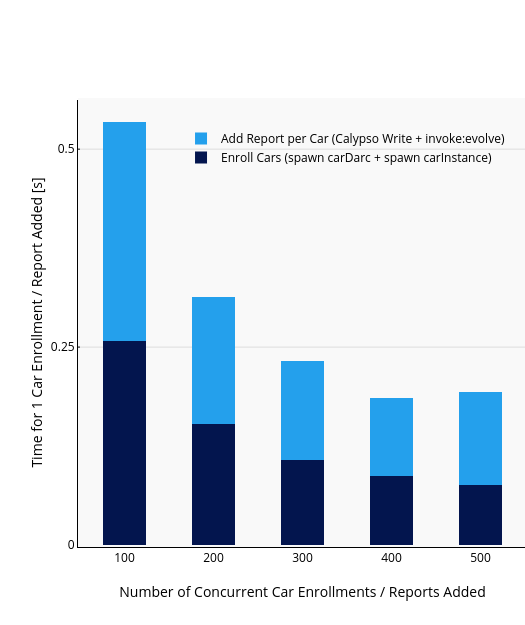
\includegraphics[width=0.65\textwidth, heigth=0.65\textwidth]{Sim/Wall-Time-Txns-Enroll.png}
    \vspace{-18pt}
    \caption{Wall Time for a Car Enrollment/Report Added with 5 Hosts}
    \label{Wall Time Txns Enroll}
\end{figure}
\begin{figure}[H]
    \centering
    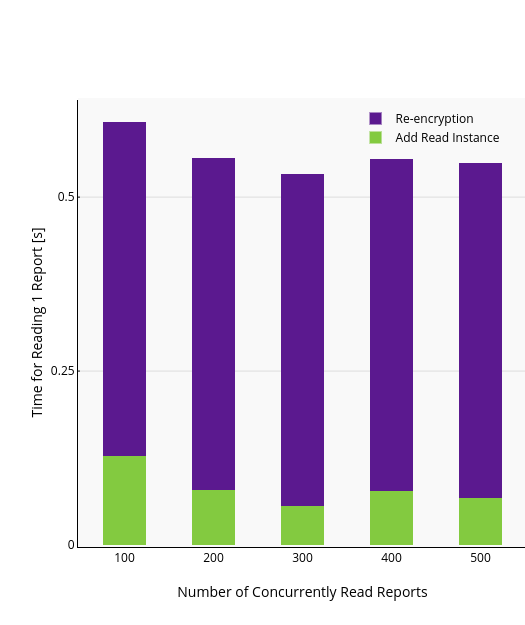
\includegraphics[width=0.65\textwidth, heigth=0.65\textwidth]{Sim/Wall-Time-Txns-Read.png}
    \vspace{-18pt}
    \caption{Wall Time for Reading a Report with 5 Hosts}
    \label{Wall Time Txns Read}
\end{figure}
\begin{figure}[H]
    \centering
    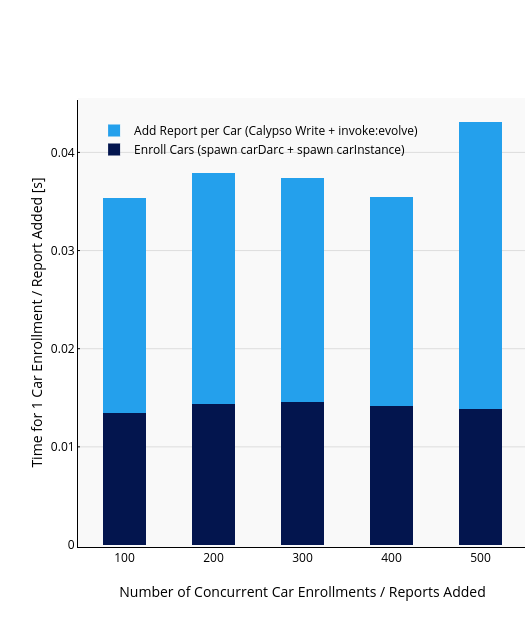
\includegraphics[width=0.65\textwidth, heigth=0.65\textwidth]{Sim/System-Cost-Txns-Enroll.png}
    \vspace{-18pt}
    \caption{System Cost for a Car Enrollment/Report Added with 5 Hosts}
    \label{System Cost Txns Enroll}
\end{figure}
\begin{figure}[H]
    \centering
    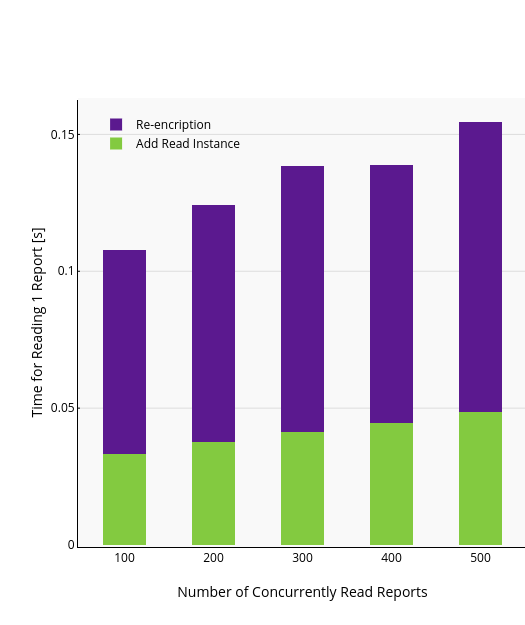
\includegraphics[width=0.65\textwidth, heigth=0.65\textwidth]{Sim/System-Cost-Txns-Read.png}
    \vspace{-18pt}
    \caption{System Cost for Reading a Report with 5 Hosts}
    \label{System Cost Txns Read}
\end{figure}



\subsection{Changing the Number of Nodes}

In this section we take into consideration a simulation where we modify the number of nodes that maintain the blockchain (5, 10, 20 and 40), whereas the number of concurrent car enrollments remains constant - 100.  The bandwidth we have configured is 100 MBps, whereas the delay between nodes is 30 ms.\\
\newline
Having performed the experiments, similarly as in the previous section, we were able to visualize the wall time (Figures~\ref{Wall Time Hosts Enroll} and~\ref{Wall Time Hosts Read}) and also the system cost (Figures~\ref{System Cost Hosts Enroll} and~\ref{System Cost Hosts Read}) measured for a single: car enrollment, report addition or reading of a report, but now in a setup with different number of hosts.\\
\newline
From all the figures in this section (Figures~\ref{Wall Time Hosts Enroll},~\ref{Wall Time Hosts Read},~\ref{System Cost Hosts Enroll} and~\ref{System Cost Hosts Read}), we can deduce that enrolling cars, adding reports and read instances in the global state, does not depend immensely on the number of hosts when there is a fixed number of simultaneous transactions. This is logically expected when every host is executing the same type of instructions.\\
\newline
What makes a big difference (for both wall time and system cost) is requesting the re-encryption key from the secret management collective authority (Figures~\ref{Wall Time Hosts Read} and ~\ref{System Cost Hosts Read}).\\
\newline
The reason behind this performance, is that in our implementation, the same nodes are utilized to form both the ByzCoin collective authority (access control) and the Calypso secret management cothority. Thus, the re-encryption process takes longer with more nodes, as the broadcasting protocol involves many members.\\
\newline
An improvement would be to use an optimal, fixed number of hosts that constitute the secret management collective authority, uncorrelated to the ones forming the access control cothority.\\
\newline
By conducting these simulations, we gained a better perspective about how our solution works in larger networks and with different number of concurrent transactions. We have also discovered limitations of the system, like not supporting 1000 simultaneous car enrollments.
\newpage
\begin{figure}[H]
    \centering
    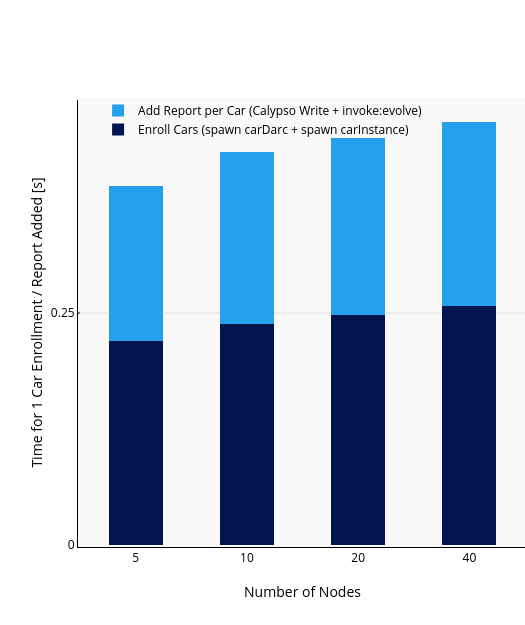
\includegraphics[width=0.65\textwidth, heigth=0.65\textwidth]{Sim/Wall-Time-Nodes-Enroll.png}
    \vspace{-20pt}
    \caption{Wall Time for a Car Enrollment/Report Added with Various Number of Nodes}
    \label{Wall Time Hosts Enroll}
\end{figure}
\vspace{-35pt}
\begin{figure}[H]
    \centering
    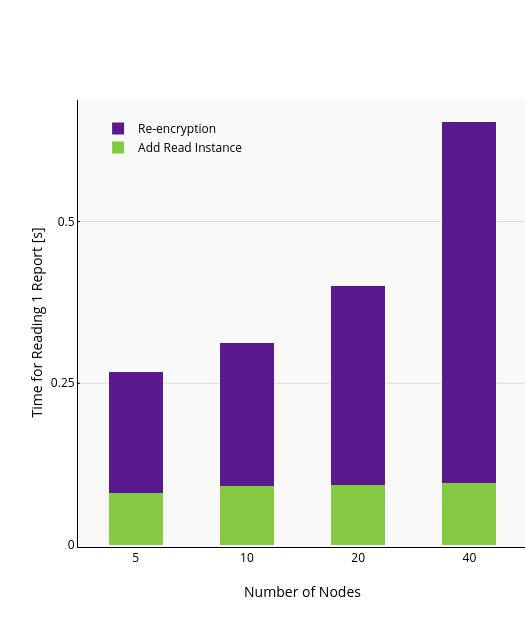
\includegraphics[width=0.65\textwidth, heigth=0.65\textwidth]{Sim/Wall-Time-Nodes-Read.png}
    \vspace{-20pt}
    \caption{Wall Time for Reading a Report with Various Number of Nodes}
    \label{Wall Time Hosts Read}
\end{figure}
\begin{figure}[H]
    \centering
    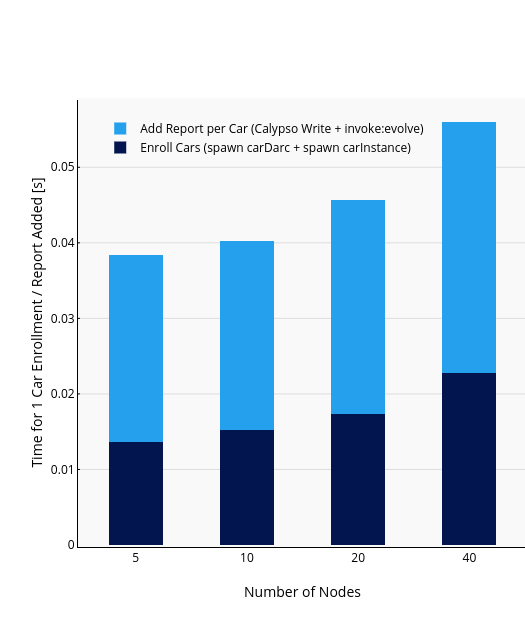
\includegraphics[width=0.65\textwidth, heigth=0.65\textwidth]{Sim/System-Cost-Nodes-Enroll.png}
    \vspace{-20pt}
    \caption{System Cost for a Car Enrollment/Report Added with Various Number of Nodes}
    \label{System Cost Hosts Enroll}
\end{figure}
\vspace{-35pt}
\begin{figure}[H]
    \centering
    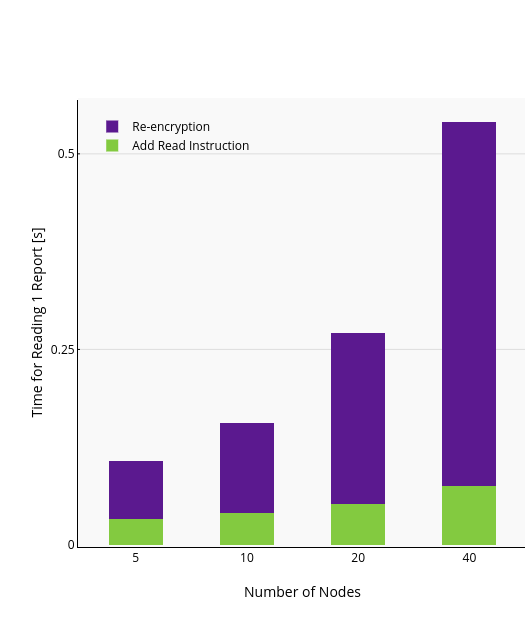
\includegraphics[width=0.65\textwidth, heigth=0.65\textwidth]{Sim/System-Cost-Nodes-Read.png}
    \vspace{-20pt}
    \caption{System Cost for Reading a Report with Various Number of Nodes}
    \label{System Cost Hosts Read}
\end{figure}


